% IPAC'27 / JACoW-style working draft.
% Official JACoW class: v3.01 (2026-03-11).
% Abstract, Introduction, and the remaining multipole-attribution study are
% intentionally left as visible placeholders until the result set is ready.
\documentclass[letterpaper]{jacow}

\usepackage[english]{babel}
\usepackage{bm}

\definecolor{draftgray}{gray}{0.95}
\newcommand{\draftplaceholder}[1]{%
  \par\smallskip
  \noindent\fcolorbox{gray}{draftgray}{%
    \parbox{0.94\columnwidth}{\textbf{DRAFT PLACEHOLDER.} #1}}%
  \par\smallskip
}

\begin{document}

\title{ORDER-DEPENDENT NONLINEAR CLOSED-ORBIT RESPONSE IN A CESR MODEL}

% TODO: Replace the temporary author metadata before circulation/submission.
\author[1]{J. N. Author\thanks{TODO: corresponding-author email}}
\affil[1]{Cornell University, Ithaca, NY, USA}

\maketitle

\begin{abstract}
  \draftplaceholder{Write after the remaining sextupole/octupole attribution
  scan is complete and the result set is frozen.}
\end{abstract}

\section{Introduction}
\draftplaceholder{Add the motivation, the relation to linear orbit-response
matrices and nonlinear closed-orbit methods, and a concise statement of the
paper's contribution after the result set is frozen.}

\section{Orbit and Optics Calculation}

A Bmad-compatible model of the Cornell Electron Storage Ring (CESR) was used
with 119 corrector variables: 58 horizontal and 61 vertical correctors.  The
orbit benchmark contains 1000 deterministic input samples, including the
zero-control reference.  The nonzero inputs are independently sampled
Gaussian corrector changes with an rms value of \qty{5}{\micro\radian},
clipped at three standard deviations.  Closed orbits are recorded at 99
zero-length detector markers in both transverse planes.

SciBmad solves the radio-frequency-on closed orbits as a batch.  A cached
$6\times119$ nominal closed-orbit response matrix supplies the initial estimate
$\bm z_0+R\Delta\bm k$; Newton iterations reuse the nominal Jacobian and send
failed lanes to a full automatic-differentiation fallback.  All 1000 formal
samples converged without fallback.  On the common \texttt{lnx201} host, the
maintained SciBmad run required \qty{33.178}{\second}, compared with
\qty{67.370}{\second} for Bmad/Tao.  The 198000 compared detector coordinates
had correlation 0.999999966 and a maximum absolute difference of
\qty{8.14}{\micro\metre}.  The latter includes differences between the
independently represented lattices and is not a Newton closure tolerance.

The associated radio-frequency-off optics benchmark evaluates periodic
coupled Twiss quantities and their first momentum derivatives at the same 99
markers.  Table~\ref{tab:calculation} summarizes representative formal results.
The parameterized calculation uses one third-order phase-space map with 119
first-order corrector parameters; it is a local surrogate rather than 1000
independent optics solutions.

\begin{table}[!htb]
  \centering
  \caption{Representative 1000-Sample Calculation Results}
  \footnotesize
  \begin{tabular}{@{}lrrr@{}}
    \toprule
    \textbf{Calculation} & \textbf{Time} & \textbf{Rate} & \textbf{Median corr.} \\
                         & \textbf{[s]}  & \textbf{[s$^{-1}$]} & \\
    \midrule
    Bmad RF-on orbit       & 67.370  & 14.843 & 1.000000 \\
    SciBmad RF-on orbit    & 33.178  & 30.140 & 1.000000 \\
    SciBmad point optics   & 570.771 & 1.752  & 1.000000 \\
    Parameterized optics   & 73.130  & 13.674 & 0.999996 \\
    \bottomrule
  \end{tabular}
  \label{tab:calculation}
\end{table}

\section{Orbit Response Error Analysis}

For corrector perturbation $\Delta\bm k$, the exact detector orbit is expanded
about the nominal machine as
\begin{equation}
  \bm u(\Delta\bm k)=\bm u_0+J\Delta\bm k
  +\frac{1}{2}H[\Delta\bm k,\Delta\bm k]
  +\frac{1}{6}T[\Delta\bm k,\Delta\bm k,\Delta\bm k]+\cdots .
  \label{eq:taylor}
\end{equation}
The residual of the nominal orbit-response approximation is
$\bm e=\bm u(\Delta\bm k)-\bm u_0-J\Delta\bm k$.  Inputs are written as
$\Delta\bm k=\rho\,\bm d\,(\qty{5}{\micro\radian})$, where every active part
of $\bm d$ has unit rms.  A sweep over 600 fixed Gaussian directions compares
all-corrector, horizontal-only, and vertical-only inputs.  It contains 36001
nonlinear states: one reference plus 20 radii, 600 directions, and three input
scenarios.  Every state converged through $\rho=12.8$.

The mean detector root-mean-square error $E(\rho)$ is calculated separately
for the horizontal and vertical detector coordinates.  Quadratic response is
diagnosed by constant $E/\rho^2$ and a local log--log slope near two.  The
small-radius coefficients in Table~\ref{tab:quadratic} show two strong
anisotropies.  First, the all-corrector horizontal residual is close to the
vertical-only value.  Second, the all-corrector vertical coefficient is about
73 times the vertical-only coefficient and 145 times the horizontal-only
coefficient.  The latter cannot be reproduced by either isolated plane and
therefore motivates a direct mixed-Hessian test.

\begin{table}[!htb]
  \centering
  \caption{Mean Quadratic Coefficients at $\rho=0.1$}
  \begin{tabular}{lrr}
    \toprule
    \textbf{Active correctors} & \textbf{$x$ residual} & \textbf{$y$ residual} \\
    & \multicolumn{2}{c}{\textbf{[$\mu$m/$\rho^2$]}} \\
    \midrule
    All              & 0.5648 & 0.5321 \\
    Horizontal only  & 0.1570 & 0.003660 \\
    Vertical only    & 0.5524 & 0.007270 \\
    \bottomrule
  \end{tabular}
  \label{tab:quadratic}
\end{table}

The all-corrector channels remain near quadratic through the complete common
range.  Horizontal-only remains near quadratic through $\rho=64$.  The clear
exception is the vertical detector residual for vertical-only inputs: it
leaves the quadratic guide around $\rho=0.28$--0.4, and its slope approaches
three while the full nonlinear reference remains converged.

\section{All-Corrector Second-Order Source}

The mixed block was isolated with 100 fixed pairs of independently sampled
horizontal and vertical corrector directions.  Each direction was normalized
to unit rms in its active family and reused at eight radii over
$0.1\leq\rho\leq1.13$.  Pure positive and negative states and all four joint
signs were evaluated, giving 6401 converged nonlinear states without fallback.
For the full detector vector,
\begin{align}
  \bm Q_{hh} &= \frac{\bm u(+\bm h,0)+\bm u(-\bm h,0)}{2}-\bm u_0,\\
  \bm Q_{vv} &= \frac{\bm u(0,+\bm v)+\bm u(0,-\bm v)}{2}-\bm u_0,\\
  \bm Q_{hv} &= \frac{\bm u(+\bm h,+\bm v)-\bm u(+\bm h,-\bm v)
  -\bm u(-\bm h,+\bm v)+\bm u(-\bm h,-\bm v)}{4}.
  \label{eq:mixedblocks}
\end{align}
Each signed quadratic residual was reconstructed as
$\bm Q_{hh}+\bm Q_{vv}+s_hs_v\bm Q_{hv}$ before taking detector rms norms.
For orbit component $u\in\{x,y\}$, the tabulated block shares are calculated for
each direction before taking percentiles,
\begin{equation}
 \begin{aligned}
 f_{ab,u}&=\frac{\lVert\bm Q_{ab,u}\rVert^2}
 {\lVert\bm Q_{hh,u}\rVert^2+\lVert\bm Q_{hv,u}\rVert^2+
  \lVert\bm Q_{vv,u}\rVert^2},\\[-1mm]
 ab&\in\{hh,hv,vv\}.
 \end{aligned}
 \label{eq:blockshare}
\end{equation}

The vertical $Q_{hv}/\rho^2$ coefficient changes by only 0.000423\% across the
fit interval.  At $\rho=1.13$, the mean vertical rms components are
\qty{0.00472}{\micro\metre}, \qty{0.00983}{\micro\metre}, and
\qty{0.71475}{\micro\metre} for $Q_{hh}$, $Q_{vv}$, and $Q_{hv}$,
respectively.  Table~\ref{tab:mixedshares} shows the distinct physical result
for the two orbit components.  For $x$, the $vv$ share has 10th, 50th, and 90th
percentiles of 61.72\%, 90.83\%, and 98.15\%.  For $y$, the corresponding
$hv$ percentiles are 99.930\%, 99.977\%, and 99.991\%.  The signed
reconstruction leaves 0.953\% of the exact vertical residual rms, while adding
$Q_{hv}$ reduces the mean squared reconstruction error by 99.982\% relative to
the pure-block reconstruction.  By contrast, the horizontal mixed share is
only 0.0146\%.  Thus the all-corrector vertical quadratic excess is a mixed
horizontal--vertical response, rather than the sum of the isolated pure-plane
terms.

\begin{table*}[!t]
  \centering
  \caption{Direction-resolved quadratic-block squared-norm shares. Each entry is median [P10, P90] in percent across the same 100 fixed H/V direction pairs. The values are invariant at the displayed precision over the verified quadratic interval.}
  \resizebox{\textwidth}{!}{%
  \begin{tabular}{@{}crrrrrr@{}}
    \toprule
    & \multicolumn{3}{c}{\textbf{X orbit component}} & \multicolumn{3}{c}{\textbf{Y orbit component}} \\
    $\rho$ & $hh$ & $hv$ & $vv$ & $hh$ & $hv$ & $vv$ \\
    \midrule
    0.1 & 9.14 [1.83, 38.26] & 0.0088 [0.0017, 0.0313] & 90.83 [61.72, 98.15] & 0.0040 [0.0007, 0.0231] & 99.977 [99.930, 99.991] & 0.0163 [0.0044, 0.0651] \\
    0.14 & 9.14 [1.83, 38.26] & 0.0088 [0.0017, 0.0313] & 90.83 [61.72, 98.15] & 0.0040 [0.0007, 0.0231] & 99.977 [99.930, 99.991] & 0.0163 [0.0044, 0.0651] \\
    0.2 & 9.14 [1.83, 38.26] & 0.0088 [0.0017, 0.0313] & 90.83 [61.72, 98.15] & 0.0040 [0.0007, 0.0231] & 99.977 [99.930, 99.991] & 0.0163 [0.0044, 0.0651] \\
    0.28 & 9.14 [1.83, 38.26] & 0.0088 [0.0017, 0.0313] & 90.83 [61.72, 98.15] & 0.0040 [0.0007, 0.0231] & 99.977 [99.930, 99.991] & 0.0163 [0.0044, 0.0651] \\
    0.4 & 9.14 [1.83, 38.26] & 0.0088 [0.0017, 0.0313] & 90.83 [61.72, 98.15] & 0.0040 [0.0007, 0.0231] & 99.977 [99.930, 99.991] & 0.0163 [0.0044, 0.0651] \\
    0.57 & 9.14 [1.83, 38.26] & 0.0088 [0.0017, 0.0313] & 90.83 [61.72, 98.15] & 0.0040 [0.0007, 0.0231] & 99.977 [99.930, 99.991] & 0.0163 [0.0044, 0.0651] \\
    0.8 & 9.14 [1.83, 38.26] & 0.0088 [0.0017, 0.0313] & 90.83 [61.72, 98.15] & 0.0040 [0.0007, 0.0231] & 99.977 [99.930, 99.991] & 0.0163 [0.0044, 0.0651] \\
    1.13 & 9.14 [1.83, 38.26] & 0.0088 [0.0017, 0.0313] & 90.83 [61.72, 98.15] & 0.0040 [0.0007, 0.0231] & 99.977 [99.930, 99.991] & 0.0163 [0.0044, 0.0651] \\
    \bottomrule
  \end{tabular}%
  }
  \label{tab:mixedshares}
\end{table*}


\section{Vertical-Corrector Signed Parity}

For a midplane-symmetric ideal lattice, reversal of the vertical-corrector
vector gives
\begin{equation}
  x(\bm v)=x(-\bm v), \qquad y(\bm v)=-y(-\bm v).
  \label{eq:selection}
\end{equation}
Consequently, the vertical detector response to vertical-only input contains
odd powers of $\bm v$.  After subtraction of the linear response, its leading
allowed nonlinear term is cubic.  By contrast, the horizontal detector
response permits a quadratic $\bm v^2$ term.  This is the closed-orbit form of
the normal-multipole midplane selection rule \cite{wolski2011}.

The order was tested directly with 100 fixed 61-dimensional vertical-corrector
directions and 27 radii.  Both signs of every direction were evaluated, giving
5401 converged nonlinear states with no fallback and a maximum one-turn closure
norm of $9.994\times10^{-14}$.  For detector plane $u$, the paired components
are
\begin{align}
  \bm e_{\mathrm{even}} &=
    \frac{\bm u(+\Delta\bm k)+\bm u(-\Delta\bm k)}{2}-\bm u_0, \\
  \bm e_{\mathrm{odd,nl}} &=
    \frac{\bm u(+\Delta\bm k)-\bm u(-\Delta\bm k)}{2}
    -J\Delta\bm k .
  \label{eq:parity}
\end{align}
Symmetric positive and negative corrector excitations are also the standard
central-difference construction used for measured orbit-response matrices
\cite{thiry2016}.

The vertical even component follows $\rho^2$, whereas the odd nonlinear
component follows $\rho^3$.  Their mean detector rms values cross at
$\rho\simeq1.31$, corresponding to an active-corrector rms kick of about
\qty{6.5}{\micro\radian}.  At $\rho=6.4$, the mean odd/even ratio is 4.91.
The horizontal detector control remains overwhelmingly even: its odd/even
ratio is $3.05\times10^{-4}$ at the same radius.

\begin{figure*}[!t]
  \centering
  \begin{minipage}[t]{0.49\textwidth}
    \centering
    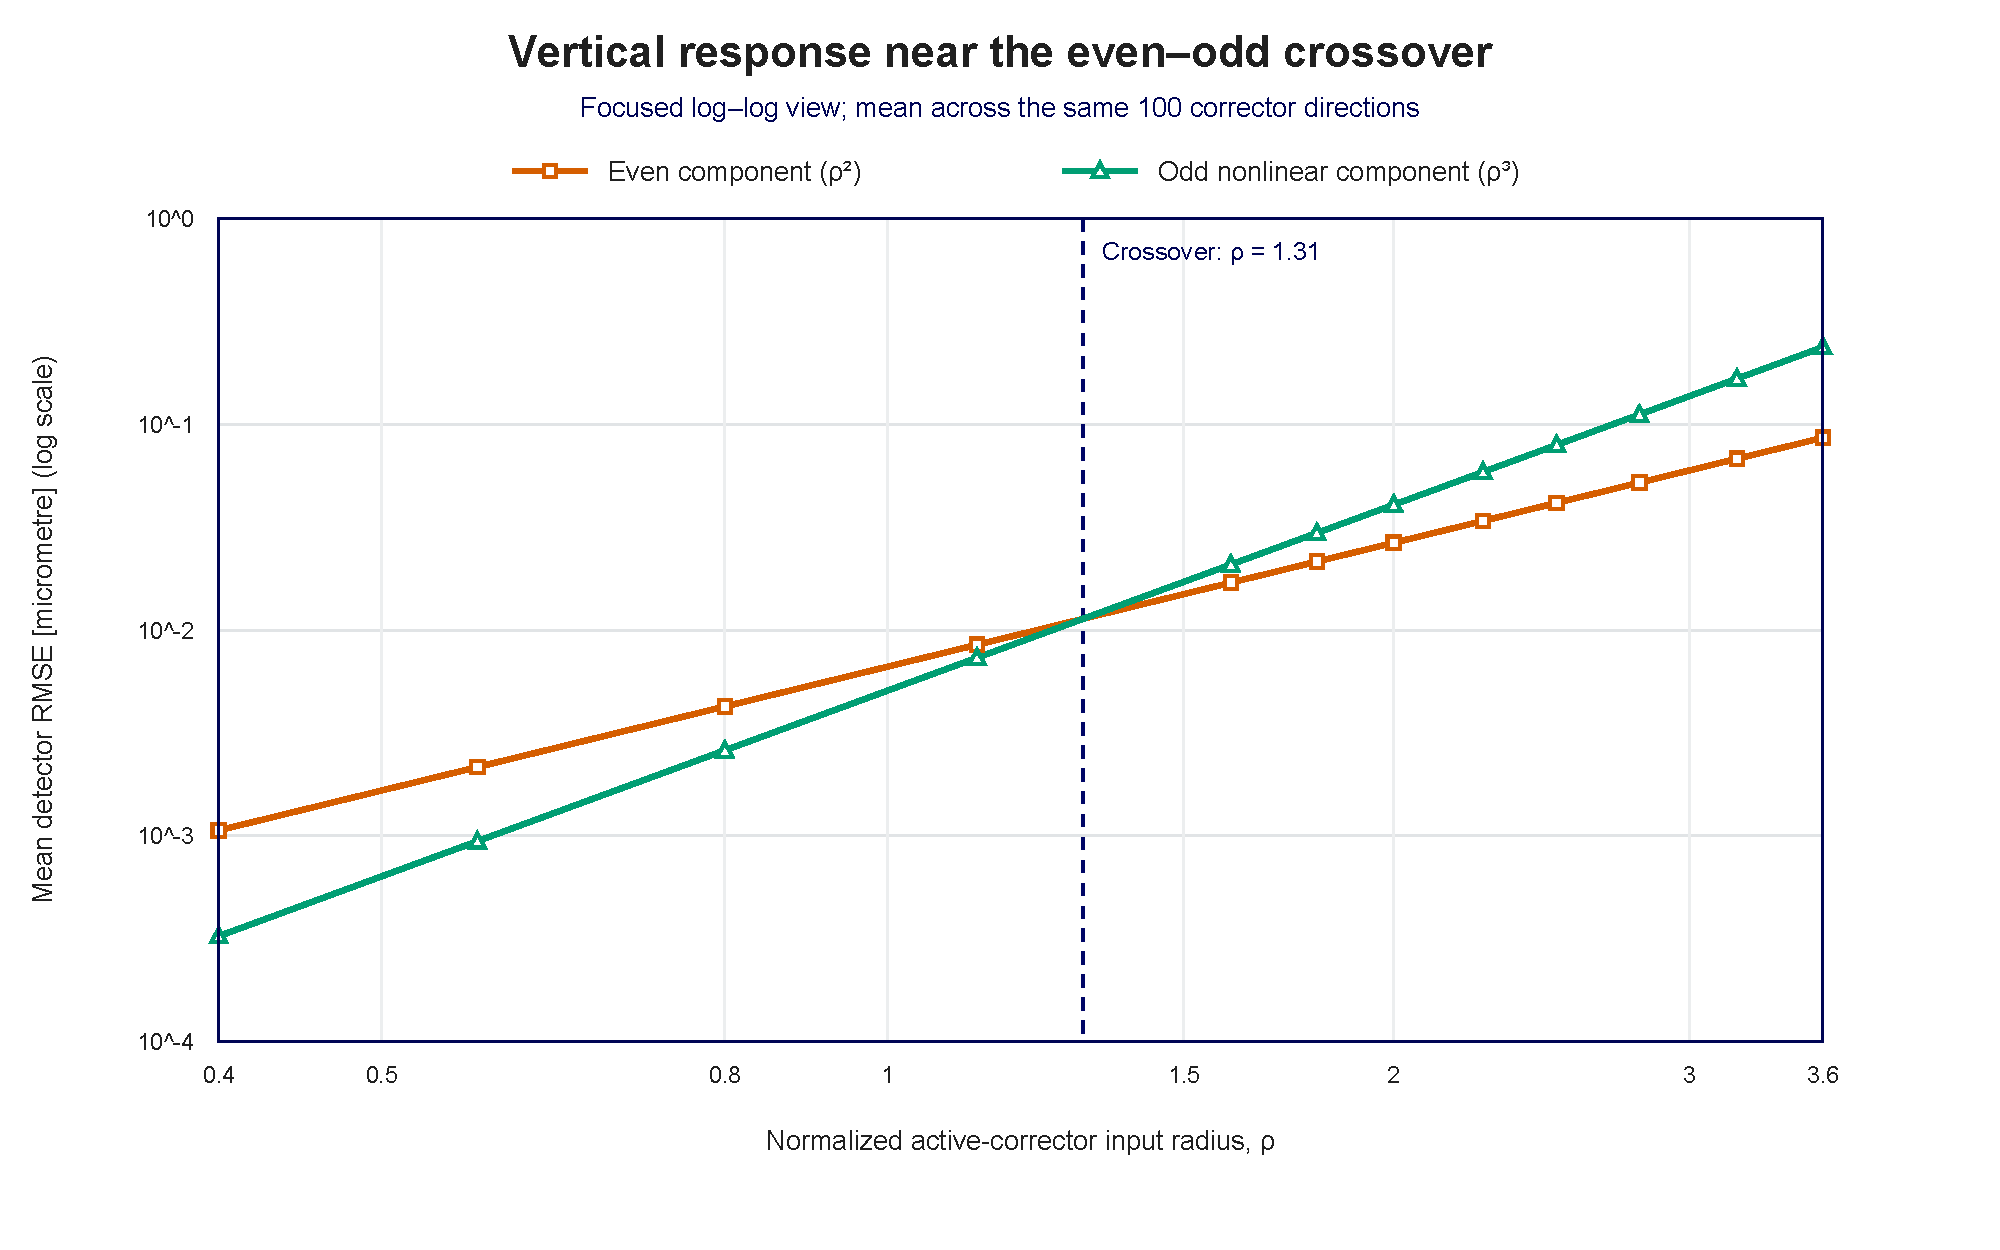
\includegraphics[width=\linewidth]{figures/vertical_parity_crossover_loglog.pdf}
    \textbf{(a)} Focused log--log crossover.
  \end{minipage}\hfill
  \begin{minipage}[t]{0.49\textwidth}
    \centering
    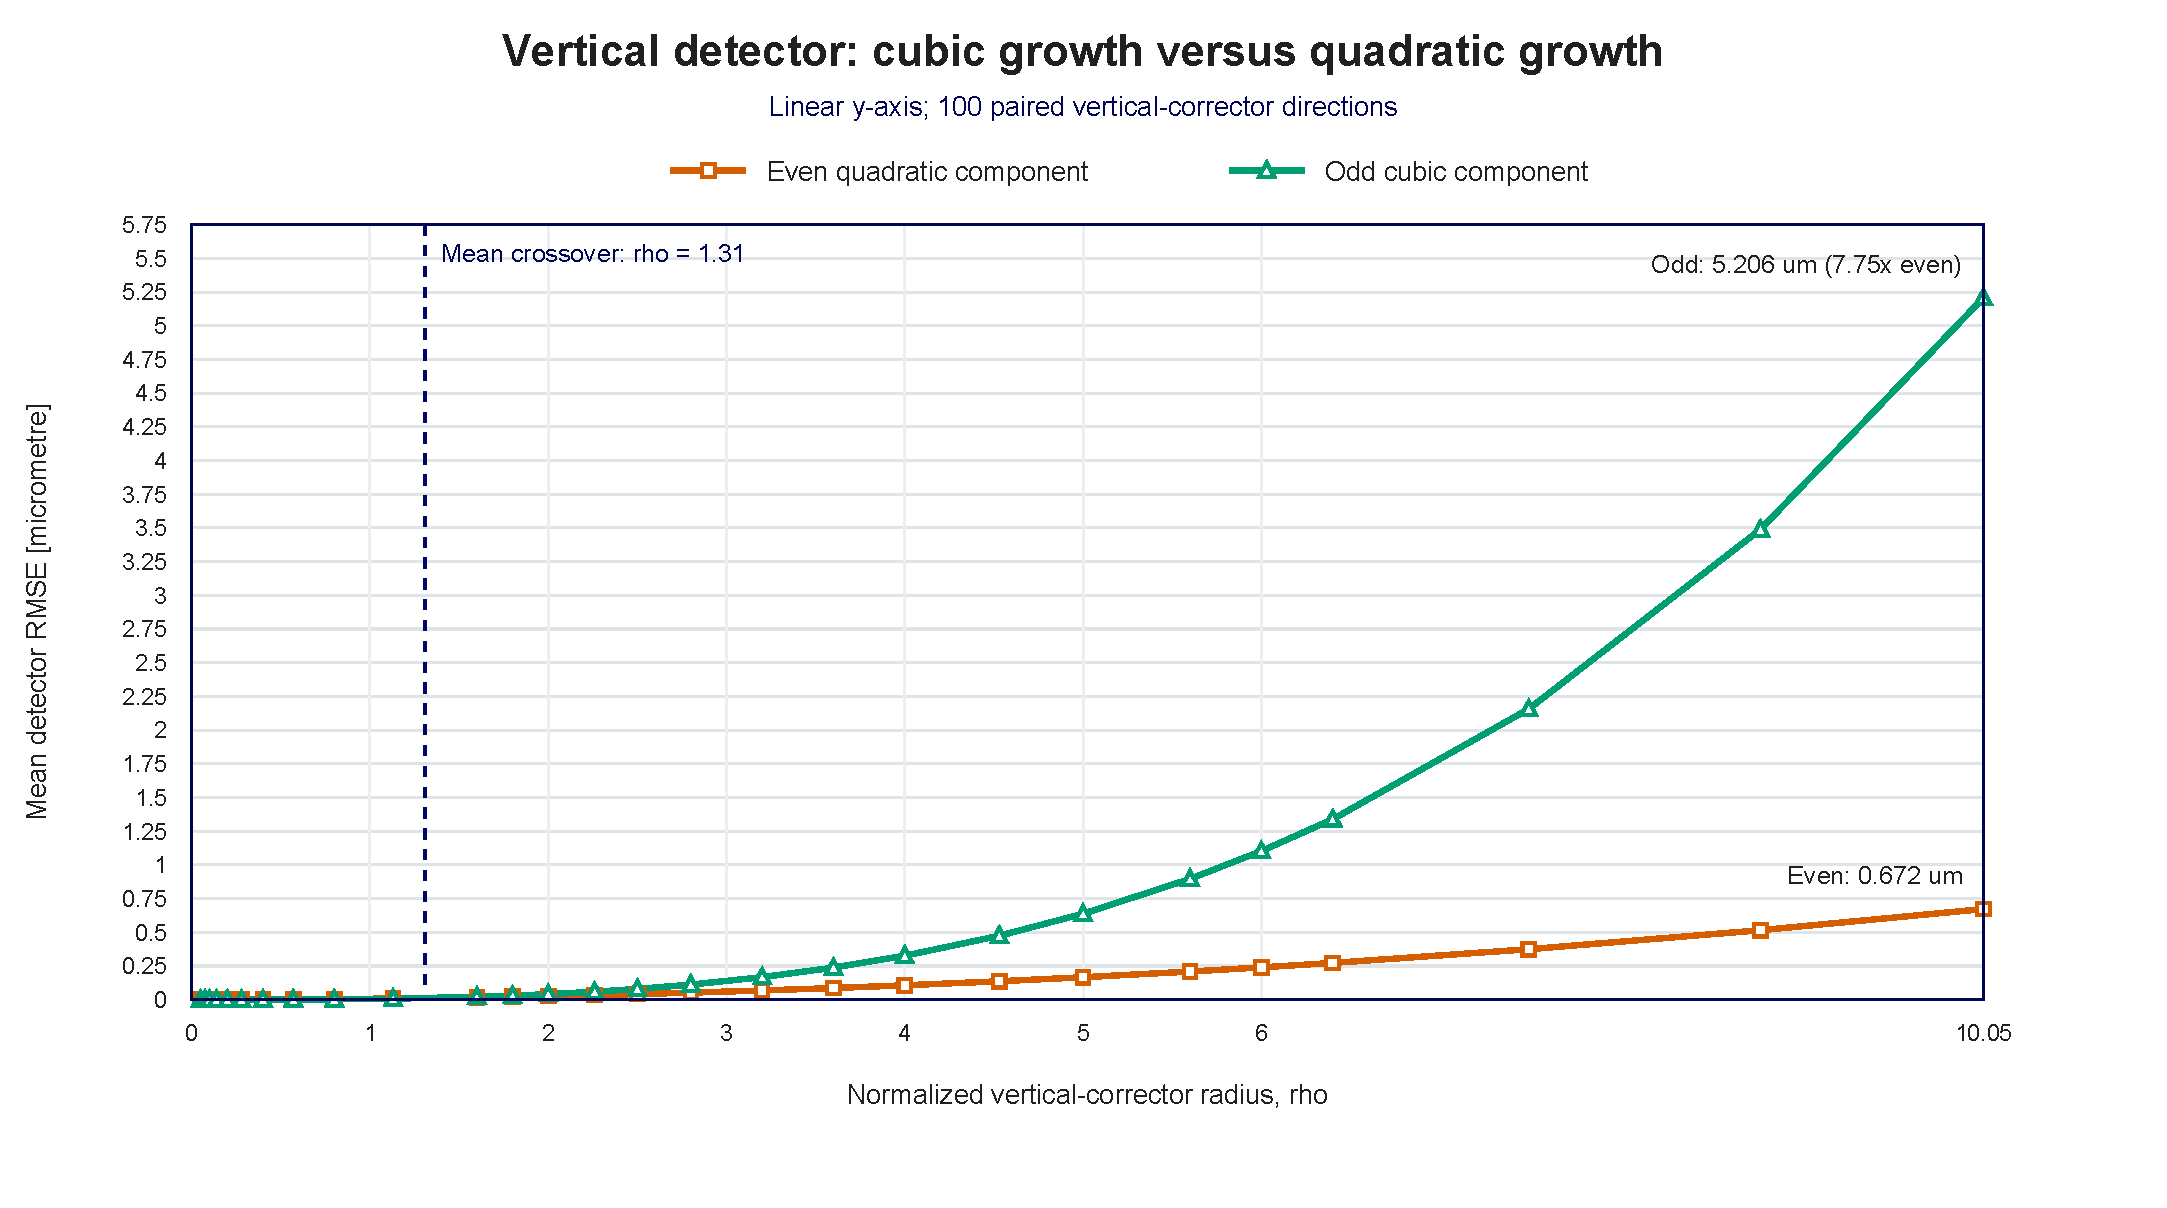
\includegraphics[width=\linewidth]{figures/vertical_parity_growth_linear.pdf}
    \textbf{(b)} Full-range linear-scale growth.
  \end{minipage}

  \vspace{1mm}
  \begin{minipage}[t]{0.62\textwidth}
    \centering
    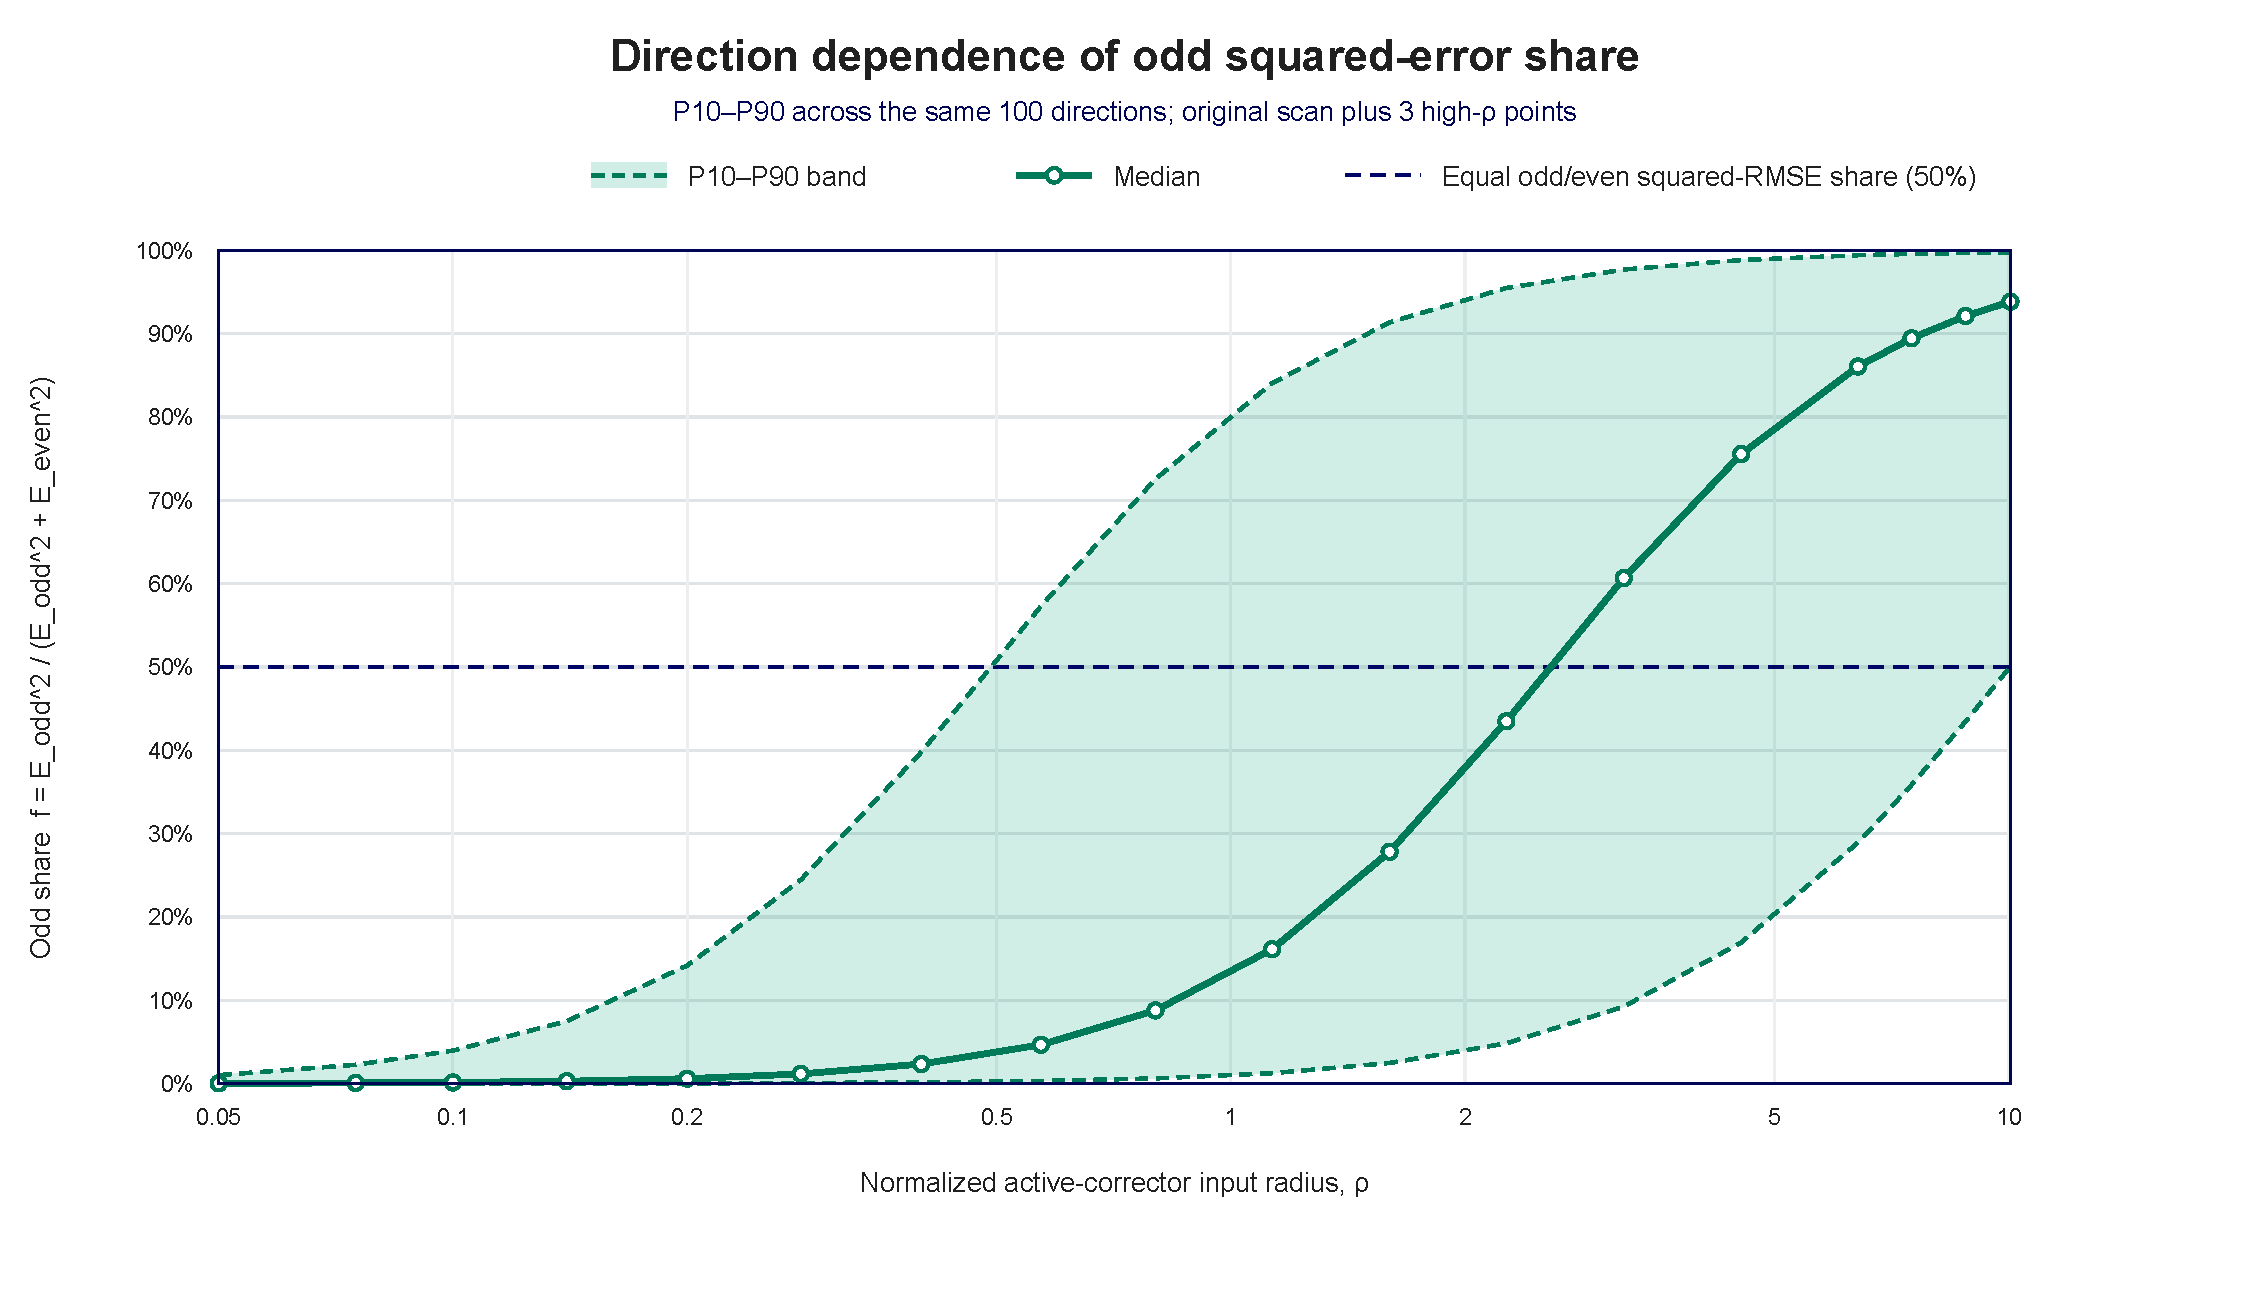
\includegraphics[width=\linewidth]{figures/vertical_parity_odd_fraction_percentiles.pdf}
    \textbf{(c)} Direction-dependent odd squared-error share.
  \end{minipage}
  \caption{Signed-parity analysis of the vertical detector residual.  The
  quadratic even and cubic odd nonlinear components cross near $\rho=1.31$.
  For each direction, the bounded odd share is
  $f=E_{\mathrm{odd}}^2/(E_{\mathrm{odd}}^2+E_{\mathrm{even}}^2)$; the band
  reports its 10th, 50th, and 90th percentiles over the same 100 directions.}
  \label{fig:parity}
\end{figure*}

The transition is direction dependent.  At $\rho=6.4$, the median odd/even
ratio is 2.48 and 80\% of directions are odd dominated.  At the extension
point $\rho=10.05$, the 10th, 50th, and 90th percentiles of $f$ are 50.06\%,
93.84\%, and 99.76\%, respectively.  Thus at least 90\% of the sampled
directions are odd dominated at that amplitude.

\subsection{Multipole attribution}

\draftplaceholder{Insert the normal-sextupole and octupole ablation/strength
scans.  Recompute the linear response for every modified lattice and fit the
direction-resolved cubic response vector, rather than comparing only one
large-amplitude rms value.  Test a sextupole-cascade scaling with $K_2^2$
against a direct octupole scaling with $K_3$, including interference if both
are significant.}

\section{Implications for Response Surrogates}

Equation~\eqref{eq:taylor} shows why one global truncation order is not
sufficient.  A quadratic Hessian is appropriate for channels whose residuals
retain $\rho^2$ scaling over the intended input distribution.  It cannot
represent the vertical-only vertical response after the odd cubic component
becomes comparable to the symmetry-breaking even term.  A practical surrogate
should therefore select order by input/output channel, retain exact nonlinear
solutions as validation references, and report its validity radius together
with direction-dependent error statistics.  Nonlinear closed-orbit and
higher-order response measurements have similarly been used to identify
sextupole behavior and other nonlinear lattice information
\cite{olsson2020,huang2024,caliari2025}.

\section{Future Optics Error Analysis}

The same order-versus-amplitude analysis will be applied to ordinary optics,
chromatic quantities, coupling observables, and orbit-derived fields.  These
classes will be reported separately because aggregation can hide a small
quadratic coefficient or an early higher-order transition.  This extension is
future work and is not used to support the orbit conclusions above.

\section{Conclusion}

The CESR-model benchmarks establish reproducible closed-orbit and optics
calculations on a shared 1000-sample input set.  The orbit-radius sweep then
identifies a channel-specific failure of a purely quadratic residual model.
Signed-direction measurements show that the vertical-only vertical residual
is an odd cubic response overtaking a small even component, rather than a
generic numerical loss of convergence.  A direction-resolved four-sign
reconstruction further separates the all-corrector quadratic source by orbit
component: the horizontal orbit is dominated by the pure vertical block
$Q_{vv}$, whereas the vertical orbit is dominated by the mixed block $Q_{hv}$.
The remaining causal test is a sextupole/octupole attribution of the cubic
coefficient.

\begin{thebibliography}{9}

  \bibitem{wolski2011}
    A. Wolski, ``Maxwell's equations for magnets'', in
    \textit{Proc. CAS 2009: Magnets}, Bruges, Belgium, Jun. 2009, pp.~1--38.
    \doi{10.5170/CERN-2010-004.1}

  \bibitem{thiry2016}
    J.-P. Thiry, A. Dieckmann, F. Frommberger, W. Hillert, and J. F. Schmidt,
    ``Lattice matching with Elegant at ELSA'', in \textit{Proc. IPAC'16},
    Busan, Korea, May 2016, pp.~2690--2692.
    \doi{10.18429/JACoW-IPAC2016-WEPOR011}

  \bibitem{olsson2020}
    D. K. Olsson, A. Andersson, and M. Sjöstr\"om,
    ``Nonlinear optics from off-energy closed orbits'',
    \textit{Phys. Rev. Accel. Beams}, vol.~23, p.~102803, 2020.
    \doi{10.1103/PhysRevAccelBeams.23.102803}

  \bibitem{huang2024}
    X. Huang, ``Correction of nonlinear lattice with closed orbit
    modulation'', in \textit{Proc. IPAC'24}, Nashville, TN, USA, May 2024,
    pp.~3054--3056. \doi{10.18429/JACoW-IPAC2024-THPC32}

  \bibitem{caliari2025}
    C. Caliari, A. Oeftiger, and O. Boine-Frankenheim,
    ``Beam-based identification of magnetic field errors in a synchrotron
    using deep Lie map networks'', \textit{Phys. Rev. Accel. Beams}, vol.~28,
    p.~024601, 2025. \doi{10.1103/PhysRevAccelBeams.28.024601}

\end{thebibliography}

\end{document}
